\begin{savequote}[75mm]
It's not the beauty of a building you should look at; it's the construction of the foundation that will stand the test of time.
\qauthor{David Allen Coe}
\end{savequote}

\chapter{Theory Overview}

\newthought{The characteristics and interactions of particles can be described by mathematical laws.} In the age of modern particle physics, there is substantial interplay between the theoretical development of these laws and their experimental validation. Experiments like those at the Large Hadron collider test initial models and experimental results are used to retune theories and construct new ones. This chapter describes those particles which have been experimentally verified and the forces and interactions which govern them. Further descriptions and a more in-depth mathematical formulation can be found in \cite{griffiths}, \cite{thomson}, \cite{schwartz}, \cite{peskin}, and \cite{srednicki}.

%% STANDARD MODEL
\section{The Standard Model}
The Standard Model (SM) of particle physics describes the fundamental particles and forces that make up all visible matter in the universe. It is considered one of the most comprehensive and powerful scientific theories ever developed due to the wide range of phenomena it describes and its predictive success. As shown in Figure \ref{fig:xc_summ}, many experimental results have been consistent with SM predictions.\\

\begin{figure}[htb!]
    \centering
    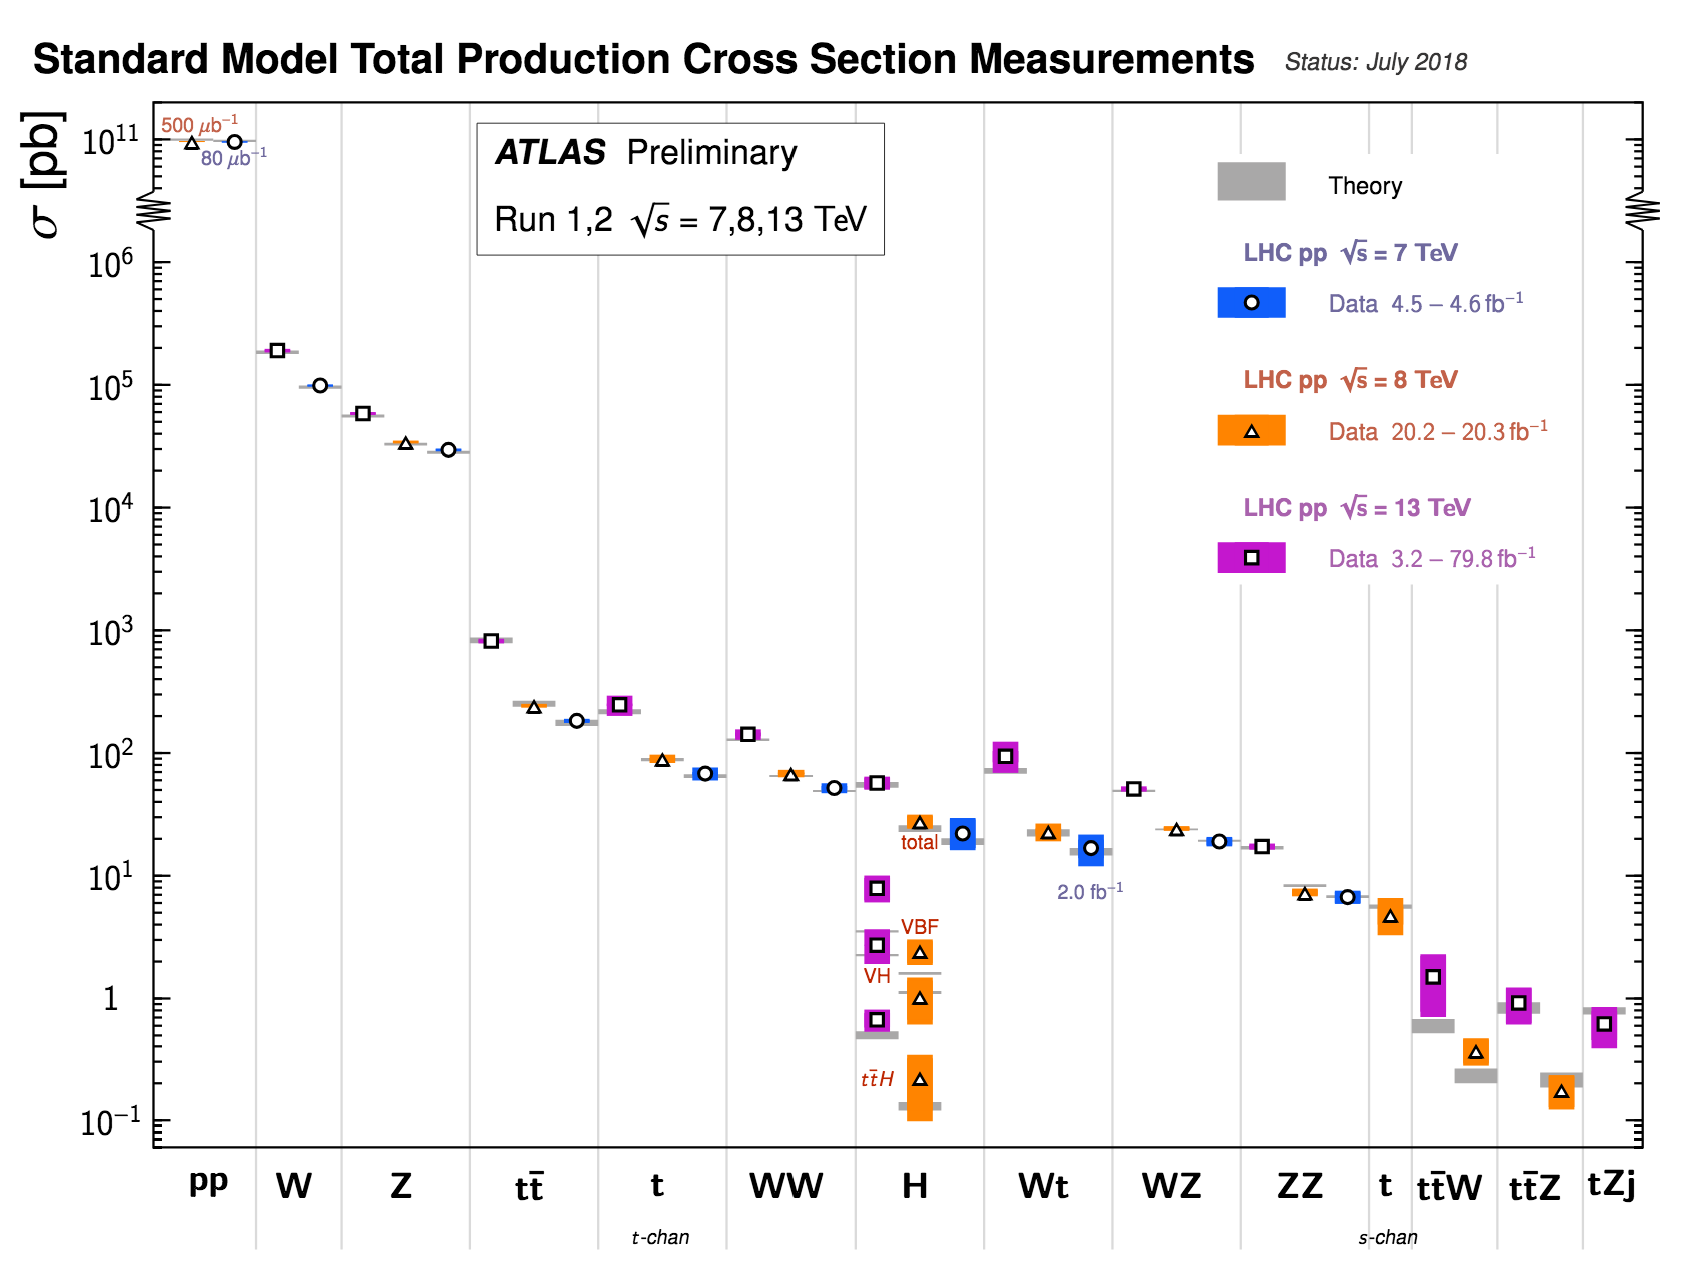
\includegraphics[width=4.5in]{figures/chapter1/sm_xc_summary.pdf}
    \caption{Summary of several SM production cross section measurements, corrected for leptonic branching fractions, and compared to the corresponding theoretical predictions \cite{sm_summary_plots}.}
    \label{fig:xc_summ}
\end{figure}

The SM particles can be summarized in a table structure (Figure \ref{fig:sm_table}), much like the Periodic Table of Elements. The particles are organized by type. For the first three columns, the top two rows describe the quarks while the bottom two rows describe the leptons; generations of particles increase from left to right. These particles are described in additional detail in Section \ref{sec:particles}. The fourth column describes the gauge bosons which mediate three of the four fundamental forces: electromagnetism, the strong force, and the weak force. These are discussed further in Section \ref{sec:forces}. Finally, the Higgs Boson is included on the far right. The Higgs couples to the quarks, bosons, and charged leptons and this interaction gives rise to particle masses. The Higgs is described in Section \ref{sec:higgs}.\\

\begin{figure}[h]
    \centering
    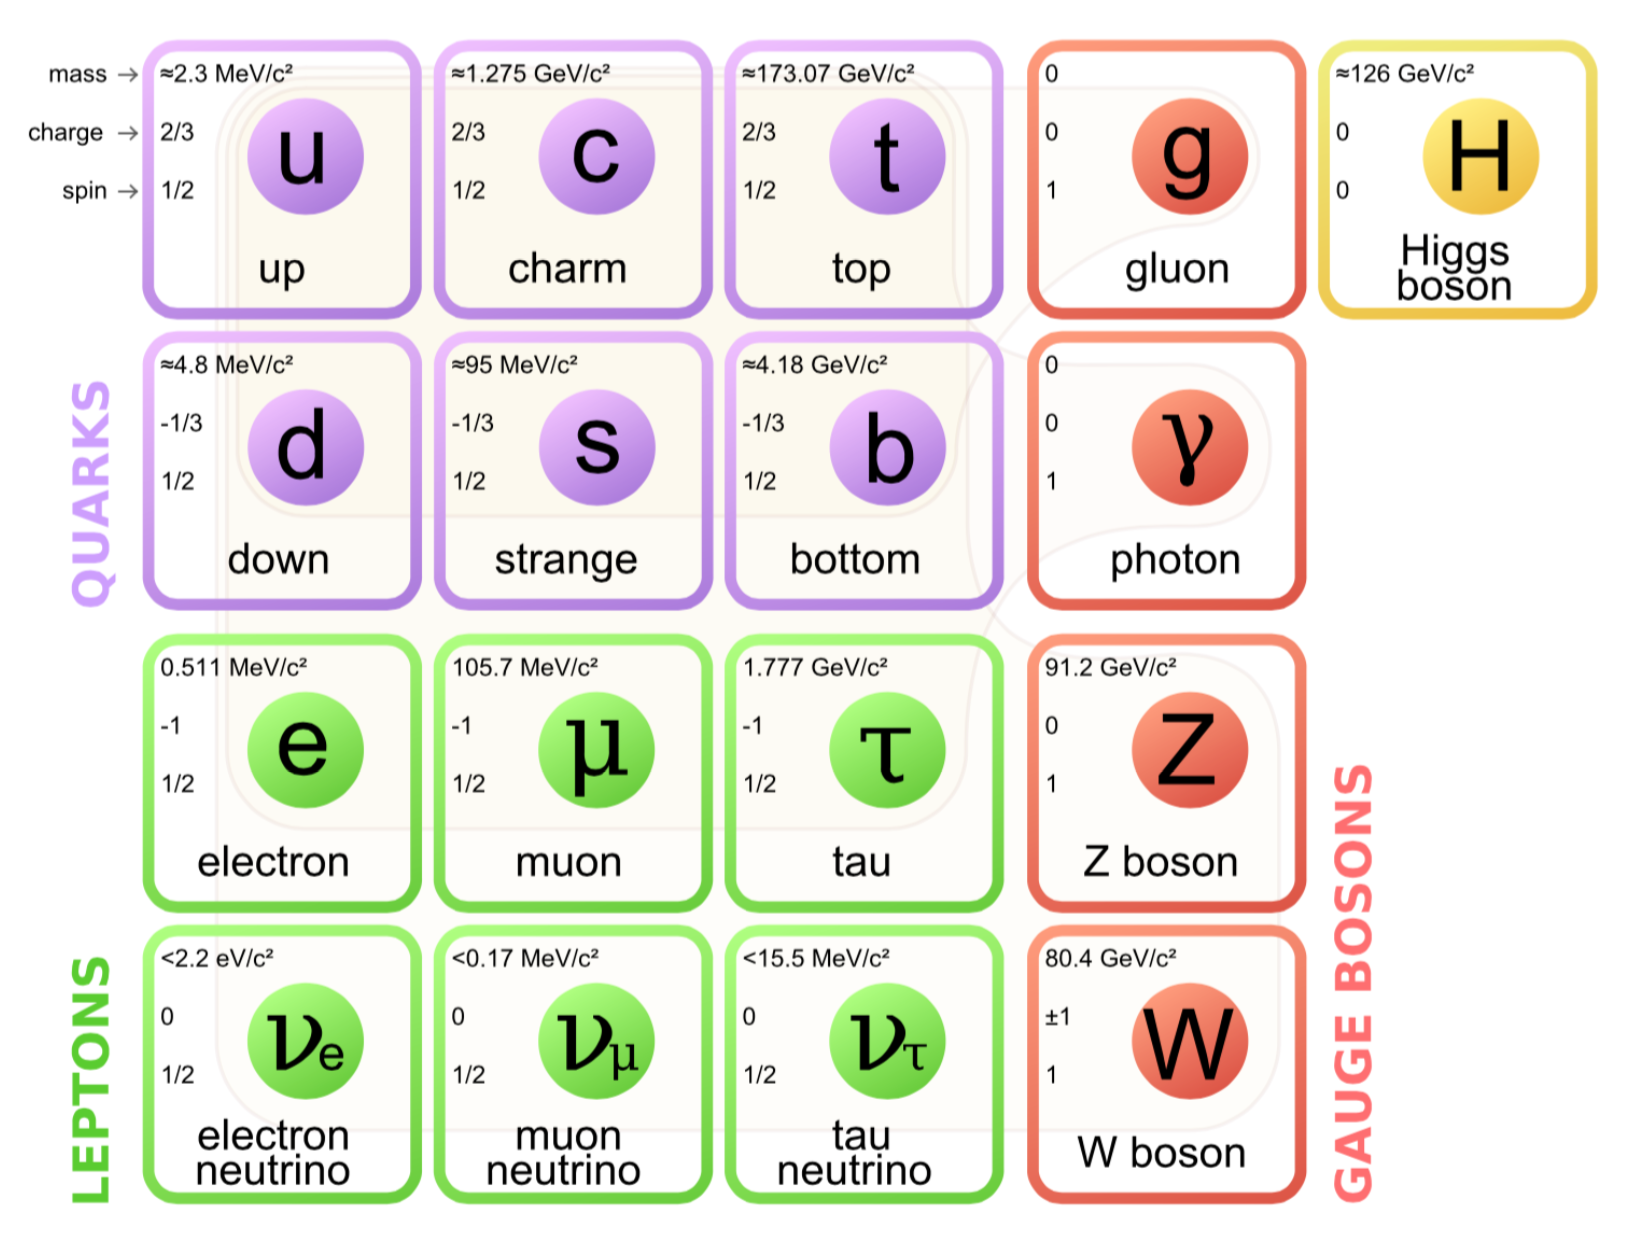
\includegraphics[width=5in]{figures/chapter1/sm.png}
    \caption{Table formation of the Standard Model which includes the mass, charge, and spin of all known SM particles.}
    \label{fig:sm_table}
\end{figure}

Although the SM has been extensively verified and has impressive predictive power, it does not fully explain all observed phenomena. For instance, there is currently no quantum theory of gravity and no explanation for the observed matter-antimatter asymmetry of the universe. Additionally, physicists have observed strong astrophysical evidence for dark matter \cite{dm_summary} and dark energy \cite{de_summary} yet the SM fails to provide any particle-based rationalization. Furthermore, within the SM itself there is no motivation for the relatively light Higgs mass (compared to the Planck mass) or the relatively large top quark mass (compared to the mass of the other 5 quarks). Collectively, these and other phenomena have motivated a robust theoretical and experimental interest in Beyond the Standard Model (BSM) physics. Many proposed BSM particles are potentially accessible at the LHC (eg \cite{bsm_hllhc}), but those theories are generally beyond the scope of this thesis.

%%subsection: particles
\subsection{Particles}\label{sec:particles}
The SM describes two types of particles: fermions and bosons. Standard quantum mechanical descriptors like mass, charge (or lack of charge), and spin are not sufficient to entirely characterize all the particles of SM, and so physicists have introduced additional quantum numbers, flavor and color, to further described internal degrees of freedom \cite{fundamental_interactions}. Additionally, as indicated by the Charge, Parity, and Time Symmetry Theorem \cite{cpt}, all SM particles have a corresponding anti-particle of the same mass but opposite charge.\footnote{This is not necessarily true for neutrinos as the SM provides no mechanism for neutrino mass creation. This is an ongoing area of study, see \cite{pdg} for additional information}\\

The fundamental SM fermions all have spin 1/2 and can be categorized by the types of interactions they experience. All fermions experience the weak force. There are six SM leptons, some of which are charged and some of which are neutral. The charged leptons are the electron ($e$), muon ($\mu$), and tau ($\tau$), which all have charge $e$ and consequently also experience the electromagnetic force. The uncharged leptons are the electron neutrino ($\nu_e$), the muon neutrino ($\nu_{\mu}$), and the tau neutrino ($\nu_{\tau}$). Due to their lack of charge they do not experience the electromagnetic force. Additionally, their masses are extremely small and are not described by the SM. All leptons are colorless and therefore do not experience the strong force.\\

There are six types of quarks: up (u), down (d), charm (c), strange (s), top (t), and bottom (b). They all carry a fractional charge which allows them to experience the electromagnetic force in addition to the weak force. Additionally, each quark carries a color charge which allows them to experience the strong force. Due to color confinement, only color neutral combinations can exist as stable particles. Consequently, quarks combine in quark-antiquark pairs called mesons and quark triplets called baryons. Mesons and baryons are collectively referred to as hadrons, the most common of which are protons and neutrons.\\

The fermions are organized into three generations. The electron, electron neutrino, up quark, and down quark form the first generation and interact to form all visible, stable, matter in the universe. The second and third generations have progressively higher mass and are unstable.\footnotemark[1] Thus far, no searches for additional generations of fermions have been successful and there is compelling indirect evidence that no further generations exist \cite{neutrino_species}.\\ 

There are four spin 1 gauge bosons in the SM: the $W^{\pm}$, the $Z^0$, the photon ($\gamma$), and the gluon ($g$). The gauge bosons are referred to as ``force carriers" because they are the particles exchanged in order to mediate the three fundamental forces in the SM. The $W^{\pm}$ and $Z^0$ are massive and mediate the weak force. Both the photon and gluon are massless; the photon mediates the electromagnetic force while the gluon mediates the strong force.

%%subsection: forces
\subsection{Forces and Interactions}\label{sec:forces}
There are four fundamental forces in nature (electromagnetic, strong, weak, and gravitational) but only three are included in the SM. There is presently no quantum formulation of gravity which is very weak at the quantum scale.\\

As described above, each of the three SM forces are mediated by a gauge boson. To first order these forces can be represented as interaction vertices between the mediating particle and the fermions which experience that force (Figure \ref{fig:vertices}). The strength of a fundamental interaction between a fermion and gauge boson is determined by the coupling constant of the interaction vertex.\\

\begin{figure}[h]
    \centering
    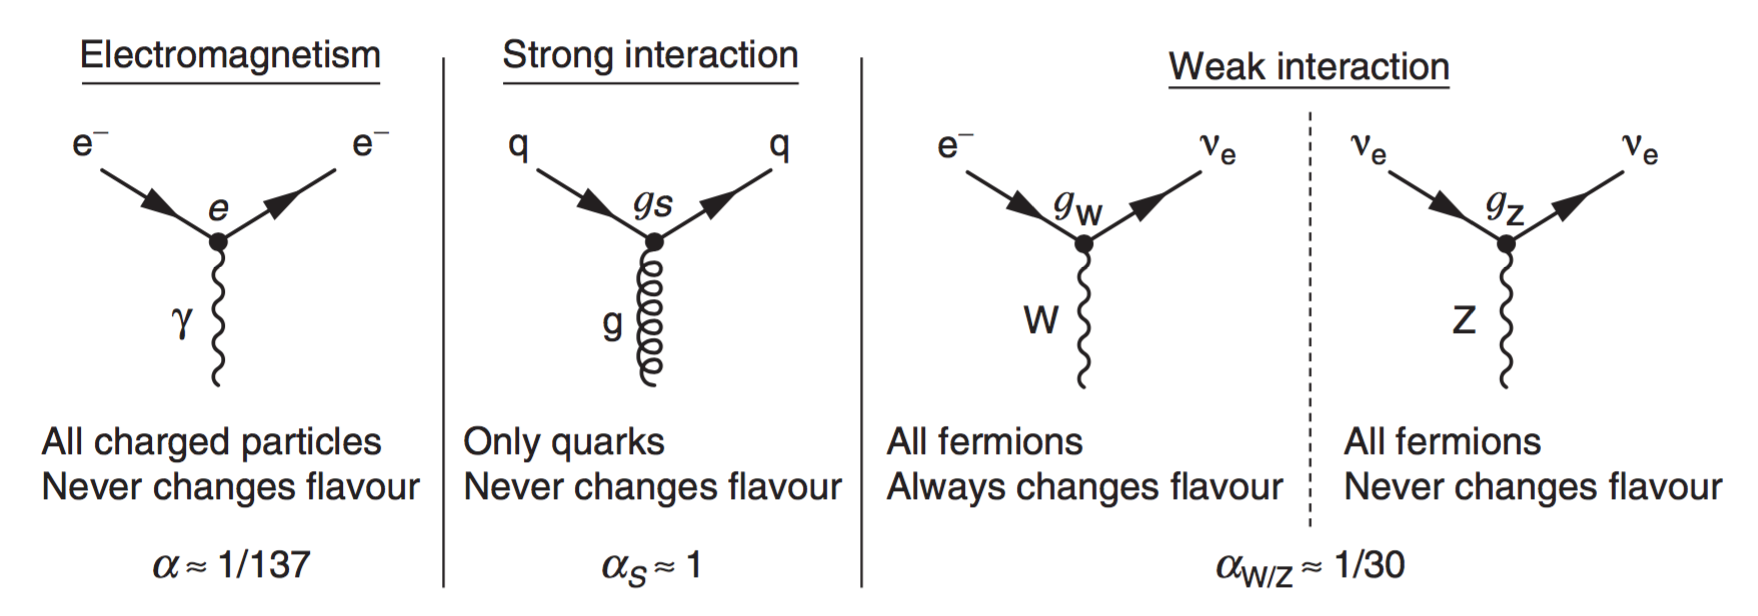
\includegraphics[width=5in]{figures/chapter1/sm_vertices.png}
    \caption{The SM interaction vertices. $\alpha$ describes the relative strength of the force as it is the dimensionless transformation of the coupling constant $g$ \cite{thomson}.}
    \label{fig:vertices}
\end{figure}

\section{Mathematical Formalism}
Mathematically, each of the three SM forces is described by a quantum field theory (QFT), where the mediating particle is treated as a vector field. These QFTs can be represented in group theory as symmetry groups which describe the invariant transformations of each force. Collectively, the SM is obeys a $SU(3)\times SU(2)\times U(1)$ group symmetry. The $SU(3)$ group arises from Quantum Chromo-dynamics (QCD), the QFT describing the strong force. The $SU(2)\times U(1)$ groups arise from Electroweak theory, the QFT which collectively describes the weak and electromagnetic forces.\\

Additionally, physicists utilize Lagrangian formalism to describe the kinetic and potential terms that regulate the interactions of these fields and their relative strengths. The Lagrangian formulations of each force begin with the the Dirac equation for the free propagation of a fermion of mass $m$: $(i\gamma^{\mu}\partial_{\mu}-m)\psi$. Here $\gamma_{\mu}=(\gamma^0,\gamma^1,\gamma^2,\gamma^3)$, the Dirac gamma matrices which satisfy the anti-commutation relations $\{\gamma^{\mu},\gamma^{\nu}\}=2g^{\mu\nu}$. $\psi$ is a spinor field solution to the Dirac equation and the Lagrangian describing $\psi$ is $\mathcal{L}=\bar{\psi}(i\gamma^{\mu}\partial_{\mu}-m)\psi$. $\bar{\psi}$ is the Dirac adjoint $\bar{\psi}=\psi^{\dagger}\gamma^0$ and $\psi^{\dagger}$ is the Hermitian conjugate. This also defines the probability density $\bar{\psi}\psi$ and the probability current $j^{\mu}=\bar{\psi} \gamma^{\mu}\psi$.\\

The mathematical formulation of each force is outlined in the following sections.\\

%% electroweak
\subsection{Electroweak}
Electroweak theory is the unification of Quantum Electrodynamics (QED), the QFT of the electromagnetic force, and the Weak theory. It represents the electromagnetic and weak forces as low energy manifestations of the same underlying force. Above the unification energy of 246 GeV, they would merge into a single electroweak force \cite{unification}.

%% QED
\subsubsection{QED}
In the development of QED the free particle Lagrangian discussed above is subject to the additional requirement of gauge invariance to spinor phase transformations: $\psi\rightarrow e^{iq\phi(x)}\psi$. This invariance is achieved by introducing the covariant derivative $D_{\mu}=\partial_{\mu}-iqA_{\mu}$. The covariant derivative includes an additional vector field $A_{\mu}$ to cancel the extra phase term in the transformed Lagrangian. In order for the Lagrangian to be fully invariant, $A_{\mu}$ must transform as $A_{\mu}\rightarrow \partial_{\mu}\phi A$.\\

Thus, the full QED Lagrangian becomes $$\mathcal{L}=\bar{\psi}i\gamma^{\mu}\partial_{\mu}\psi - m\bar{\psi}\psi - q\bar{\psi}\gamma^{\mu}A_{\mu}\psi - \frac{1}{4}\mathcal{F}^{\mu\nu}\mathcal{F}_{\mu\nu}.$$

\noindent Here $\mathcal{F}^{\mu\nu}=\partial^{\mu}A^{\nu} - \partial^{\nu}A^{\mu}$ is the  anti-symmetric gauge invariant electromagnetic field strength tensor. The first term in the Lagrangian is the fermionic kinetic term, the second term is the fermion mass term, the third term is the interaction term, and the final term is the kinetic term for the $A_{\mu}$ field. The field kinetic term can be understood in terms of classical electromagnetic theory as giving rise to the electric and magnetic fields: $-\frac{1}{4}\mathcal{F}^{\mu\nu}\mathcal{F}_{\mu\nu}=\frac{E^2-B^2}{2}$.\\

The gauge field $A_{\mu}$ is mediated by the photon. According to the Lagrangian, the photon must be massless as including as mass term for $A_{\mu}$ would violate gauge invariance. Additionally, QED is an abelian gauge theory which prohibits any photon self-interaction terms. QED is represented by the $U(1)$ gauge group symmetry.

%% WEAK
\subsubsection{The Weak Interaction}\label{sec:weak}
Dirac spinors can be decomposed into two irreducible representations called left-handed and right-handed Weyl spinors:
$\psi=\begin{pmatrix}\psi_L \\ \psi_R \end{pmatrix}$. The projections of a Dirac spinor onto its left and right states are obtained by the operators $P_L=\frac{1-\gamma^5}{2}$ and $P_R=\frac{1+\gamma^5}{2}$ respectively. Here $\gamma^5$ is the matrix:
$$\gamma^5=i\gamma^0\gamma^1\gamma^2\gamma^3= \begin{pmatrix} -\mathbb{I}_2 && 0\\ 0 && \mathbb{I} \end{pmatrix}.
$$

The Weyl spinors behave the same under rotation transformations but experience opposite transformations under Lorentz boosts. The operation of flipping the signs of spatial coordinates is referred to as Parity (P). Invariance under parity transformations, also called chiral symmetry, is an important property in QFT. The Weyl spinors can be connected through a parity transformation as $P(\psi_{R/L}(t,\vec{x}))=\psi_{L/R}(t,-\vec{x})$.\\

Historically, many physicists believed parity would be conserved in all particle interactions. However the 1957 observation of $\beta$-decay in polarised Cobalt-60 demonstrated that partiy was in fact not conserved in the weak interaction. This indicates that the weak interaction vertex and corresponding probability current must have a different form than that of QED.\\

While any bilinear covariant derivative can be used to construct SM Lagrangian terms, experimental data indicated the need for both vector currents and parity violating axial currents in equal parts to fully explain $\beta$-decay. Thus the weak interaction vertex could take the form of either $\gamma^{\mu}(1-\gamma^5)$ or $\gamma^{\mu}(1+\gamma^5)$. Experimentally it was shown that the weak charged current is a vector minus axial (V-A) interaction with a coupling vertex factor $-ig'/2\sqrt{2}\times\gamma^{\mu}(1-\gamma^5)$ where $g'$ is the weak coupling constant. The left projection operator $P_L$ appears in the vertex factor indicating that only the left-handed chiral component of fermions interact with the charged weak force.\\

This formulation of the weak force is represented by the $SU(2)_L$ local gauge symmetry group. $SU(2)$ is generated by the Pauli matrices $\sigma^a/2$ for $a=\{1,2,3\}$. This introduces three massless vector fields $W_{\mu}^a$ which can be combined to form the fields of the physically observable $W^{\pm}$ bosons as $W^{\pm}_{\mu}=\frac{1}{\sqrt{2}}(W_{\mu}^1\mp iW_{\mu}^2)$. The remaining field $W_{\mu}^3$ is an independent neutral weak field. $SU(2)_L$ is a non-abelian group which allows $W^{\pm}$ self-interactions.

%%Unification
\subsubsection{Electroweak Unification}\label{sec:ew}
The Glashow model of electroweak unification replaces the general $U(1)$ symmetry of QED with a new $U(1)_Y$ local gauge group which is symmetric under the transformation $\psi(x)\rightarrow exp[ig'\frac{Y}{2}\zeta(x)]\psi(x)$. This gives rise to a new gauge field $B_{\mu}$ which couples to the new ``weak hypercharge", Y, rather than the electromagnetic charge e.\\ 

Electroweak unification describes the mixing of this new $B_{\mu}$ field with the weak neutral field $W^3$ by introducing the new covariant derivative $D_{\mu}=\partial_{\mu}-ig\sigma^a W_{\mu a}+ig'\frac{1}{2}YB_{\mu}$. In order to preserve full $SU(2)_L\times U(1)_Y$ symmetry, the $W_{\mu}^a$ and $B_{\mu}$ fields have strength tensors $W^{a\mu\nu}=\partial^{\mu}W^{a\mu}-\partial^{\nu}W^{a\mu}+gf^{abc}W^{b\mu}W^{c\nu}$ and $B_{\mu\nu}=\partial_{\mu}B_{\nu}-\partial_{\nu}B^{\mu}$ respectively. In the equation for the $W_{\mu}^a$ field strength tensor, $f$ is the totally anti-symmetric structure constant. Finally, this leads to the unified electroweak Lagrangian:
\begin{multline}\nonumber
\mathcal{L}=-\frac{1}{4}B^{\mu\nu}B_{\mu\nu} - \frac{1}{4}W^{a\mu\nu}W_{a\mu\nu} \\ + \bar{\psi}_L\gamma^{\mu}(\partial_{\mu}-ig\frac{\sigma^a}{2}W_{\mu}^a+ig'\frac{1}{2}YB_{\mu})\psi_L + \bar{\psi}_R\gamma^{\mu}(\partial_{\mu}+ig'YB_{\mu})\psi_R.
\end{multline}

The fields of the physically observable neutral $Z^0$ boson and photon can be written as mixed states of the $W_{\mu}^3$ and $B_{\mu}$ fields. The corresponding mixed fields are  $Z_{\mu}=W_{\mu}^3cos\theta_W - B_{\mu}sin\theta_W$ and $A_{\mu}=W_{\mu}^3sin\theta_W + B_{\mu}cos\theta_W$ respectively. Here, $\theta_W$ is the Weinberg weak mixing angle which is related to the coupling strengths of the electromagnetic and weak force as $cos\theta_W=\frac{g}{\sqrt{g^2+g'^2}}$. $\theta_W$ is a free parameter in the SM which can be constrained experimentally.\\

Fermionic mass terms like $m\bar{\psi}\psi$ seen in the original formulation of QED are no longer allowed as the electroweak Lagrangian treats left and right Weyl spinors differently. Additionally, the four electroweak gauge bosons must be massless to preserve gauge symmetry of the Lagrangian. It is clear in nature that some SM fermions and bosons do in fact have mass, and this seeming contradiction is reconciled by the Higgs field described in Section \ref{sec:higgs}.

%% QCD
\subsection{QCD}\label{qcd}
QCD is the QFT of the strong force. The strong force is only experienced by quarks which carry an additional quantum number called color. Thus, QCD is subject to the additional constraint that color charge is conserved. There are three color quantum numbers referred to as red, blue, and green, and so QCD is based on the $SU(3)_C$ symmetry group.\\

The QCD Lagrangian must be invariant under gauge transformations of the form $U=\exp(-i\sum_{j=1}^8{\theta_j\lambda_j/2})$ where $\theta_j$ are arbitrary parameters and $\lambda_j$ are the Gell-Mann matrices. This requires the introduction of the covariant derivative $D_{\mu}=\partial_{mu}+ i\alpha_S t_i G_{\mu}^i$ where $G_{\mu}^i$ are the 8 gluon fields (which mediate the strong force) and $\alpha_S$ is the gluon field coupling strength. The strength tensor of the gluon field is $\mathcal{G}_{\mu\nu i}=\partial_{\mu}G_{\nu i}-\partial_{\nu}G_{\mu i}+\alpha_S f_{ijk}G_{\mu j}G_{\nu k}$ where $f_{ijk}$ are the $SU(3)$ structure constants and $t_i=\lambda_i/2$.\\ 

The full QCD Lagrangian is then
$$
\mathcal{L}=-\frac{1}{4}\mathcal{G}^i_{\mu\nu}\mathcal{G}^{i\mu\nu}+\bar{\psi}_{fa}(i\gamma^{\mu}\partial_{\mu}\delta_{ab}-\alpha_S\gamma^{\mu}t^i_{ab}G^i_{\mu}-m_f\delta_{ab})\psi_{fa}.
$$
Here, $f$ labels quark flavor ($f\in[1,6]$), $a$ labels color, $i\in[1,8]$ indexes the gluons, and $t^i_{ab}$ are the generators of $SU(3)$ which satisfy the commutation relation $[t_a,t_b]=if_{abc}t_c$. QCD is a non-abelian theory which allows for gluon self-interactions.\\

%%THE HIGSS
\section{The Higgs Boson}\label{sec:higgs}
This mathematical description of the SM, as presented above, is not self-consistent. The physically observed masses of the gauge bosons break the gauge symmetry of the $SU(2)_L \times U(1)_Y$ electroweak interaction. The Brout-Englert-Higgs mechanism, described further in Section \ref{sec:ews_sm}, was proposed in 1964 to spontaneously break electroweak symmetry (EWS) \cite{higgs_higgs} \cite{higgs_brout} \cite{higgs_guralnik}. This mechanism also predicted the existence of a spin 0 scalar particle, generally referred to as the Higgs boson or simply the Higgs.\\

A Higgs-like particle with a mass of 125 GeV was discovered by the ATLAS and CMS experiments in 2012 \cite{higgs_disc_atlas} \cite{higgs_disc_cms}. Thus far, all measurements of this particle have been consistent with the SM and the Brout-Englert-Higgs mechanism of EWS breaking (ESWB). This result solidifies physicists' understanding of how bosons and fermions acquire mass and places constraints on some free parameters of the SM. The study of the Higgs continues to be a high priority research area at the LHC as verifying all of its production and decay modes and measuring any self-couplings is critical to further understand its role in the SM.

%%subsection: ew symmetry breaking
\subsection{Electroweak Symmetry Breaking}\label{sec:ews_sm}
In order to keep the mathematical description of the SM renormalizable EWS must be broken spontaneously, meaning the SM Lagrangian is invariant under the electroweak transformation but the individual spinor states are not. The mathematical mechanism of EWSB is introduced below and described in further detail in \cite{higgs_physics_notes}.\\

To spontaneously break EWS, a new complex scalar field $\Phi$ is introduced. To preserve the invariance of the EW Lagrangian, $\Phi$ must be an $SU(2)_L\times U(1)_Y$ multiplet; the simplest multiplet, the isospin dublet:
$$
\Phi=\begin{pmatrix}\Phi^+ \\ \Phi^0\end{pmatrix} = \frac{1}{\sqrt{2}} \begin{pmatrix}\Phi_1+i\Phi_2 \\ \Phi_3+i\Phi_4\end{pmatrix}
$$
can be used to represent the new field. The Lagrangian of the new field is $\mathcal{L}=(D^{\mu}\Phi)^{\dagger}(D_{\mu}\Phi)-V(\Phi)$ where $D_{\mu}$ is the covariant derivative of EWS and $V(\Phi)$ is the potential of the scalar field. The potential of the Higgs field is $V(\Phi)=\mu^2\Phi^2+\lambda\Phi^4$. Requiring $\lambda>0$ and $\mu^2<0$ allows a physical solution with spontaneous symmetry breaking as shown in Figure \ref{fig:higgs_potent} as the true minimum of the potential is given by $\Phi^2_{min}=\frac{-\mu^2}{\lambda}$.

\begin{figure}[h]
    \centering
    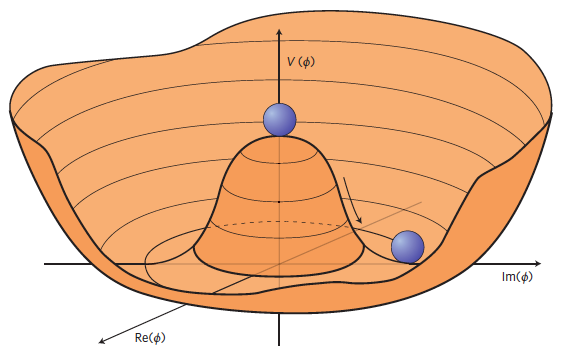
\includegraphics[width=4in]{figures/chapter1/higgs_potential.png}
    \caption{An illustraion of the Higgs potential in the case that $\mu^2<0$ \cite{higgs_physics_notes}.}
    \label{fig:higgs_potent}
\end{figure}

This minimization of $\Phi^2$ in fact defines a circle of infinite degenerate solutions, and without loss of generality one can chose the intuitive representation $\Phi_1=\Phi_2=\Phi_4=0$ and $\Phi_3=v=\sqrt{-\mu^2/\lambda}$. Here, $v$ is the vacuum expectation value of the Higgs field. Thus, the field can be written as $$\Phi_{vacuum}=\frac{1}{\sqrt{2}}\begin{pmatrix}0 \\ v\end{pmatrix}.$$.

The resulting particle spectrum can be understood by examining the Lagrangian under small perturbations from the minimum of the form $\Phi=\frac{1}{\sqrt{2}}\begin{pmatrix}0 \\ v+h\end{pmatrix}$. Consider the kinetic term for the Higgs field $(D^{\mu}\Phi)^{\dagger}(D_{\mu}\Phi)$:
\begin{gather*}
D_{\mu}\Phi=\frac{1}{\sqrt{2}}[ig\frac{1}{2}\sigma^aW_{\mu a}+ig'\frac{1}{2}YB_{\mu}] \begin{pmatrix}0 \\ v+h\end{pmatrix}\\
= \frac{i}{2\sqrt{2}}[g(\begin{pmatrix} 0 & W_1 \\ W_1 & 0\end{pmatrix} + \begin{pmatrix} 0 & -iW_2 \\ iW_2 & 0\end{pmatrix} + \begin{pmatrix} W_3 & 0 \\ 0 & -W_3\end{pmatrix})+ g'\begin{pmatrix} YB_{\mu} & 0 \\ 0 & YB_{\mu}\end{pmatrix}] \begin{pmatrix} 0 \\ v+h\end{pmatrix}\\
= \frac{i(v+h)}{2\sqrt{2}} \begin{pmatrix}g(W_1-iW_2) \\ -gW_3+g'YB_{\mu}\end{pmatrix}
\end{gather*}
and so
$$
(D^{\mu}\Phi)^{\dagger}(D_{\mu}\Phi)=\frac{(v+h)^2}{8}[g^2(W_1^2+W_2^2)+(-gW_3+g'YB_{\mu})^2].
$$
A new orthonormal basis for the Lagrangian can be defined in terms of the fields of the physically observable $W^{\pm}_{\mu}$, $Z_{\mu}$, and $A_{\mu}$ bosons defined in Sections \ref{sec:weak} and \ref{sec:ew}. Finally, the Higgs Lagrangian becomes:
\begin{align*}\nonumber
& \mathcal{L} = \frac{1}{2}\partial_{\mu}h\partial^{\mu}h - \lambda v^2h^2 \\
& + \frac{1}{2}(\frac{g'^2v^2}{4}((W^+_{\mu})^2+(W^-_{\mu})^2) +  \frac{v^2}{4}(g^2+g'^2)Z^2_{\mu} + 0\cdot A^2_{\mu}) \\
& + \frac{g^2v}{4}((W^+_{\mu})^2+(W^-_{\mu})^2)h + \frac{g^2}{8}((W^+_{\mu})^2+(W^-_{\mu})^2)h^2 \\
& \frac{v^2}{4}(g^2+g'^2)Z_{\mu}^2h = \frac{1}{8}(g^2+g'^2)Z_{\mu}^2h^2 \\
& - \lambda v h^3 - \frac{\lambda}{4}h^4.
\end{align*}

Here the first line of the Lagrangian gives the kinetic and mass terms of the Higgs field, the second line gives the mass terms of the $W^{\pm}$ and $Z^0$ bosons, the third line gives the coupling of the $W^{\pm}$ bosons to the Higgs field, the fourth line gives the coupling of the $Z^0$ boson to the Higgs field, and the final line gives the self-interaction terms of the Higgs.  This formulation of the Lagrangian defines the masses of the gauge bosons as
$$
m_{W^{\pm}}=\frac{1}{2}vg, \; \; \; \; \; m_Z=\frac{1}{2}v\sqrt{g^2+g'^2}.
$$
Additionally, it defines the Higgs mass as $m_H=v\sqrt{2\lambda}$. It is clear that there are no mass or Higgs coupling terms for the $A_{\mu}$ photon fields and thus the photon remains massless.

%%subsection: yukawa
\subsection{Yukawa Coupling}\label{sec:yukawa}
The mass of SM fermions is described through their Yukawa couplings. The Yukawa interaction describes how fermionic Dirac spinor $\psi$ interfaces with the scalar Higgs field $\Phi$. This can be expressed mathematically as a cubic interaction of the form $g_Y\bar{\psi}\Phi\psi$ where $g_Y$ is the Yukawa coupling constant. The Lagrangian for this interaction is then $\mathcal{L}=\frac{1}{2}D^{\mu}\Phi D_{\mu}\Phi-V(\Phi)+\bar{\psi}(iD_{\mu}\gamma^{\mu}-m)\psi - g_Y\bar{\psi}\Phi\psi.$ Expanding the interaction term using the specific Higgs potential described above yields fermionic mass terms of the form 
$$ m_i\bar{\psi_i}\psi_i=\frac{g_{Y,i}v}{\sqrt{2}}.
$$
The individual Yukawa couplings $g_{Y,i}$ are free parameters in the SM that can be constrained experimentally. 

%subsection: production methods
\subsection{Higgs Production Methods}\label{sec:higgs_prod}
There are four main Higgs production mechanisms that can be studied using proton-proton collisions at the LHC. All four have now been observed and the measured production cross-sections are consistent with SM predictions. Each mode is introduced briefly below and Figure \ref{fig:higgs_prod} shows the SM production cross-sections for a $\sqrt{s}=13$TeV proton-proton collider as a function of the Higgs mass. 

\begin{figure}[h]
    \centering
    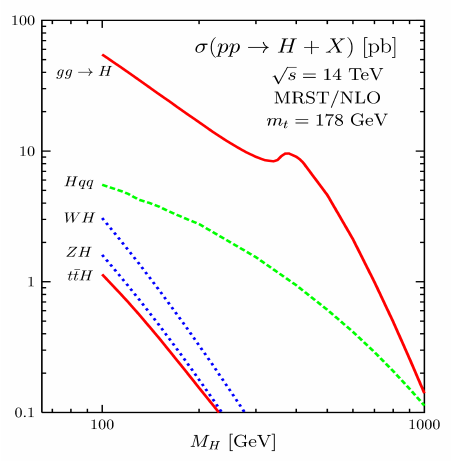
\includegraphics[width=3in]{figures/chapter1/higgs_prod.png}
    \caption{Dominant SM Higgs production cross-sections as a function of Higgs mass \cite{higgs_prod_fig}.}
    \label{fig:higgs_prod}
\end{figure}

\subsubsection{Gluon-Gluon Fusion}\label{sec:ggf}
As shown in Figure \ref{fig:higgs_prod}, gluon-gluon fusion (ggf) is the dominant production mode for the 125 GeV Higgs. The ggF process must occur through a quark loop, as demonstrated in Figure \ref{fig:ggf}, because the Higgs only couples to massive particles. As shown in Section \ref{sec:yukawa}, the Higgs-fermion cupling strength increases with fermion mass and thus the quark loop is most often a top or bottom loop. This production mode has been observed for multiple Higgs decay modes and contributed substantially to the initial Higgs discovery \cite{higgs_disc_atlas}.

\begin{figure}[h]
    \centering
    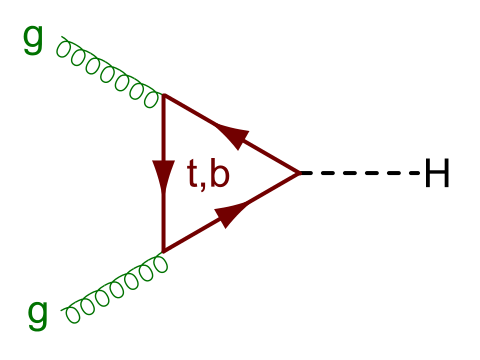
\includegraphics[width=2in]{figures/chapter1/ggf.png}
    \caption{Feynman diagram of gluon-gluon fusion Higgs boson production with a top or bottom quark loop}
    \label{fig:ggf}
\end{figure}

\subsubsection{Vector Boson Fusion}
The second most common Higgs production mode at the LHC is Vector Boson Fusion (VBF). This process is shown to first order in Figure \ref{fig:vbf}. VBF is quark initiated; the quarks within the colliding protons exchange virtual $W^{\pm}$ or $Z^0$ and this exchange emits a Higgs. The interacting quarks do not need to be the same type which increases the cross-section of this process. As with ggF, VBF production has been observed for multiple Higgs decay modes and was central to the Higgs discovery \cite{higgs_disc_atlas}.

\begin{figure}[h]
    \centering
    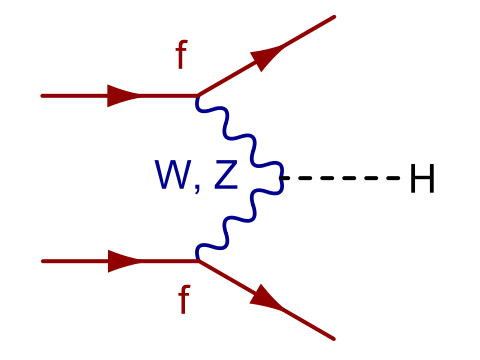
\includegraphics[width=2in]{figures/chapter1/vbf.png}
    \caption{Feynman diagram of vector boson fusion Higgs boson production}
    \label{fig:vbf}
\end{figure}

\subsubsection{Associated Production with a Vector Boson}
The next most common Higgs production mode, and the focus of the analysis described in Chapters 6 and 7, is associated production of the Higgs with a $W^{\pm}$ or $Z^0$ boson. This process, shown in Figure \ref{fig:vh}, is commonly referred to as VH where V represents vector boson. The leading production process is quark initiated; a quark and anti-quark merge to form a virtual $W^{\pm}$ or $Z^0$ which, if sufficiently energetic, then radiates a Higgs. As shown in Figure \ref{fig:higgs_prod}, the WH cross-section is slightly larger than the ZH cross-section due to the lower mass of the W. 

\begin{figure}[h]
    \centering
    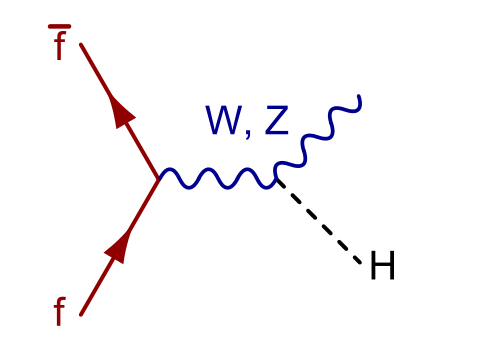
\includegraphics[width=2in]{figures/chapter1/vh.png}
    \caption{Feynman diagram of associated Higgs boson production with a vector boson}
    \label{fig:vh}
\end{figure}

\subsubsection{Top Fusion}
The final relevant production mode is top fusion, ttH. As shown in Figure \ref{fig:tth}, ttH is gluon initiated and each initial gluon decays into a top anti-top pair (two of which then fuse to form the Higgs). Due to the high mass of the top quark, this production mechanism requires a large amount of energy and consequently has the lowest cross-section. The ttH mode was observed independently in 2018 \cite{tth}. 

\begin{figure}[h]
    \centering
    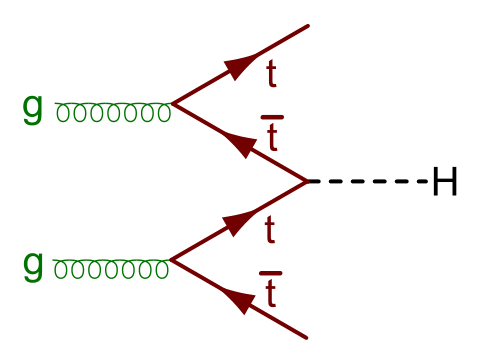
\includegraphics[width=2in]{figures/chapter1/tth.png}
    \caption{Feynman diagram of top fusion Higgs boson production}
    \label{fig:tth}
\end{figure}

%subsection: decays
\subsection{Higgs Boson Decays}
As shown in Sections \ref{sec:ews_sm} and \ref{sec:yukawa}, the Higgs couples to all massive SM particles, except neutrinos, and thus there are many potential decay modes for the Higgs. Although incorporating SM conservation laws of charge, color, and flavor reduces that number somewhat, there are still numerous allowed decays. The main Higgs decays accessible at a $\sqrt{s}=13$TeV collider are summarized in Figure \ref{fig:higgs_br}. The likelihood of each decay, referred to as the branching ratio (BR), depends on the particle's coupling strength to the Higgs, the differences in mass, and the mass of the Higgs itself. Each of these decay modes is introduced briefly below and additional information, including second-order-decay-product-influenced measurement strategies, can be found in \cite{pdg}.\\

\begin{figure}[h]
    \centering
    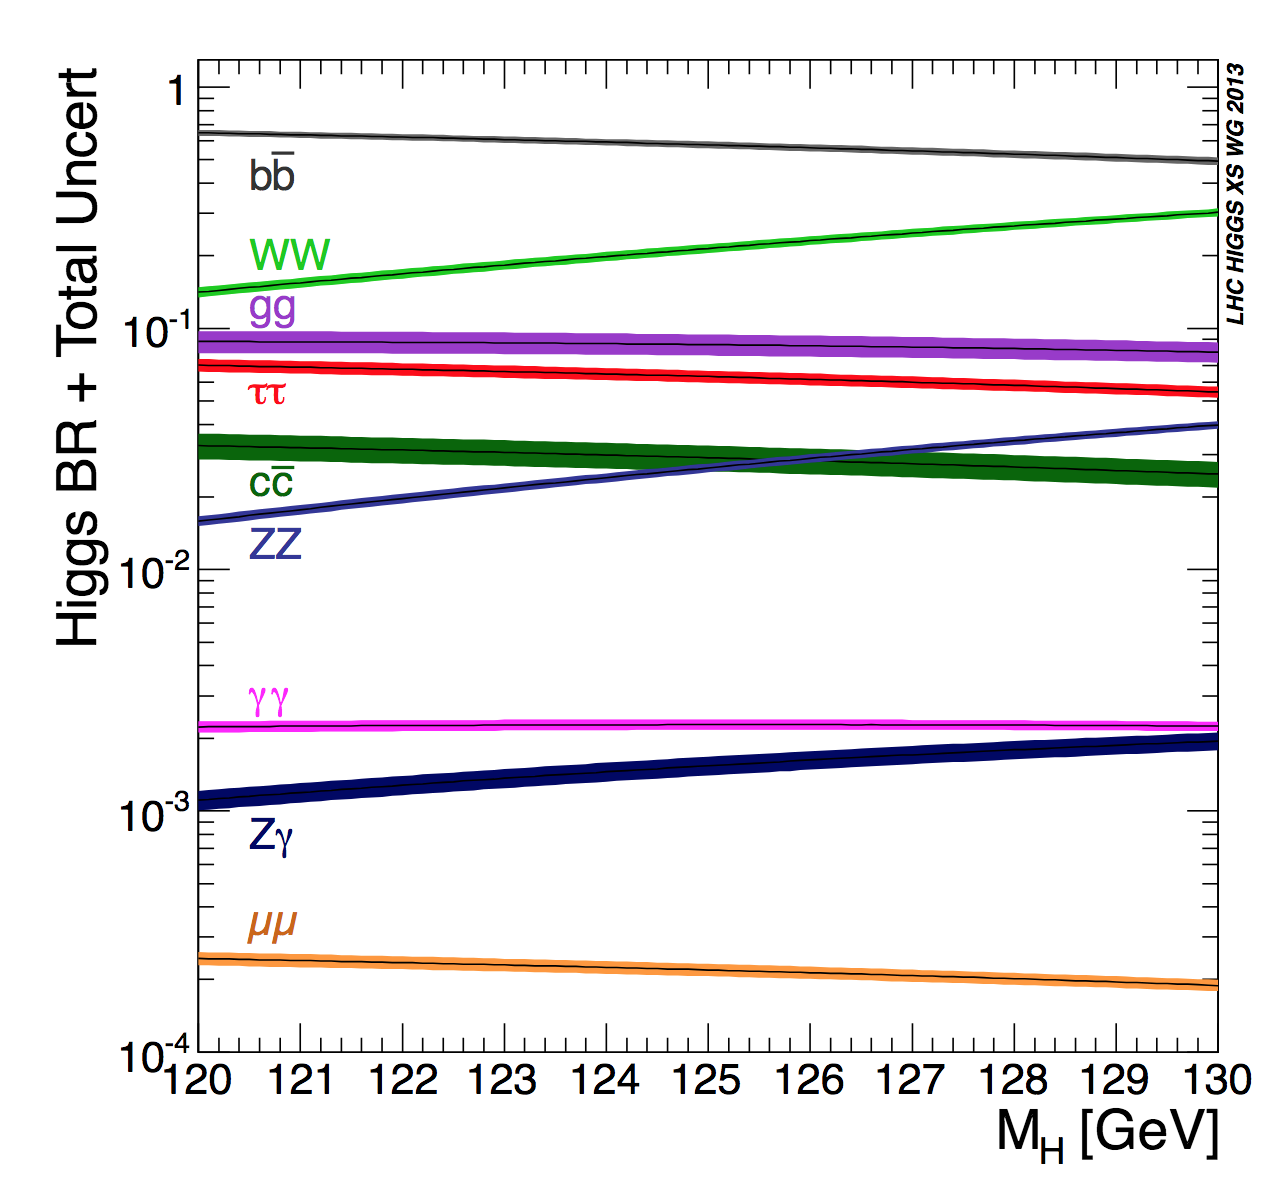
\includegraphics[width=4in]{figures/chapter1/higgs_brs.png}
    \caption{Branching ratios for the main decays of a SM Higgs boson as a function of Higgs mass. The theoretical uncertainties are shown as bands \cite{pdg}.}
    \label{fig:higgs_br}
\end{figure}

\subsubsection{Massive Fermions}
One way for the Higgs to decay is into a fermion-antifermion pair. As derived in Section \ref{sec:yukawa}, the fermionic Higgs coupling strengths are proportional to the fermion masses and thus decays to heavy fermions have a higher BR. A decay to a top-antitop pair is disallowed for a 125GeV Higgs due to mass constraints, and so the most common Higgs decay is to a bottom-antibottom pair. This decay has a BR of 0.584. Despite being the most likely Higgs decay mode, it was not observed independently until Run 2 due to difficulties triggering on, reconstructing, and identifying b-quarks \cite{higgs_bbar}.The next most common quark-antiquark decay is to a charm-anticharm pair which has a BR of 0.029. This decay mode has not been independently observed \cite{higgs_ccbar}. Higgs decays to lighter quarks have a BR too low for observation at the LHC.\\

The most likely leptonic decay of the Higgs, and the subject of the analysis described in Chapters 6 and 7, is to a $\tau^+\tau^-$ pair due to the relatively high tau mass. The BR for this decay is 0.0627 and it has been observed for three of the four production modes described in Section \ref{sec:higgs_prod} \cite{higgs_tautau}. Higgs decay to a $\mu^+\mu^-$ pair has a BR of only 0.000218 which positions it as the least likely decay mode for feasible observation at the LHC. Measuring this decay channel is an important goal for the HL-LHC \cite{higgs_hllhc}. The BR for Higgs to an $e^+e^-$ is generally believed to be too low for potential observation at the LHC.\\

\subsubsection{Massive Bosons}
Additionally, the Higgs may split into a pair of massive gauge bosons. The BR for Higgs to $W^+W^-$ is 0.214, making it the second most common Higgs decay. It was initially observed for the ggF and VBF production modes in Run 1 \cite{higgs_ww1} and for ttH \cite{tth} and VH \cite{vh_ww} production in Run 2. The BR for Higgs to a $ZZ$ pair is substantially lower at only 0.0262. However, the $H\rightarrow ZZ \rightarrow llll$ channel, often referred to as the `golden channel', has a very clean signature due to the presence of four leptons and thus was one of the initial Higgs discovery channels \cite{higgs_disc_atlas}.

\subsubsection{Massless Particles}
The Higgs may also decay into massless gauge bosons (photons and gluons), but these processes require an intermediate loop of virtual heavy quarks or massive bosons. The $H\rightarrow gg$ is the most likely of these decays with a BR of 0.086. Gluons carry color charge and thus this decay must be mediated by a quark loop, most often a top loop. This decay is in fact the inverse of the ggF production mode described in Section \ref{sec:ggf}. This decay is difficult to measure at colliders.\\ 

The Higgs decay to two photons ($\gamma\gamma$) may proceed through fermion or boson loops and has a much smaller BR, only 0.0027. However, like the $H\rightarrow ZZ \rightarrow llll$, it is a feasible signature to measure at colliders due to excellent photon momentum reconstruction and identification. This decay was also one of the initial Higgs discovery channels \cite{higgs_disc_atlas}. A decay to $Z\gamma$ is also allowed in the SM, with a BR of 0.00154 and requires a virtual massive fermion or boson loop similar to the $\gamma\gamma$ decay. This decay mode has not yet been observed \cite{higgs_zgam}.\\

The SM does not provide a mechanism for generating neutrino masses, but there are multiple BSM extensions that predict Higgs decays to neutrinos. Many of these theories create signatures that are potentially observable at LHC detectors; see for example \cite{higgs_neutrino1} and \cite{higgs_neutrino2}.

